\documentclass{article}
\usepackage{amsmath}
\usepackage{amssymb}
\usepackage{graphicx}

% redefine \VerbatimInput
\usepackage[dvipsnames]{xcolor}
\usepackage{fancyvrb}
\RecustomVerbatimCommand{\VerbatimInput}{VerbatimInput}%
{fontsize=\footnotesize,
 %
 frame=lines,  % top and bottom rule only
 framesep=2em, % separation between frame and text
 rulecolor=\color{Gray},
 %
 label=,
 labelposition=topline,
 %
}

\usepackage[top=1in, bottom=1.25in, left=1.25in, right=1.25in]{geometry}

\newcommand{\mtwotwo}[4]{\begin{bmatrix} #1 & #3 \\ #2 & #4 \end{bmatrix}}
\newcommand{\br}[1]{\left\{#1\right\}}
\newcommand{\brkt}[1]{\left[#1\right]}
\newcommand{\prn}[1]{\left(#1\right)}
\newcommand{\reals}{\mathbb{R}}
\newcommand{\cyc}[1]{\mathbb{Z}_{#1}}
\newcommand{\ints}{\mathbb{Z}}
\newcommand{\rationals}{\mathbb{Q}}
\newcommand{\lcm}{\text{lcm}}
\newcommand{\galois}[1]{\mathbb{F}_{#1}}

\begin{document}
\title{\textbf{COSC363 -- Assignment 2 -- Ray tracing}}
\author{Lucas Payne --- 73231707}
\date{}
\maketitle

\newcommand{\thing}[3]{
\vskip 0.2in
\hrule
\vskip 0.03in
\hrule
\vskip 0.1in
    \textbf{\textit{#3 #1}}:
#2
\vskip 0.1in
\hrule
\vskip 0.03in
\hrule
\vskip 0.2in
}
\newcommand{\feature}[2]{\thing{#1}{#2}{Feature}}
\newcommand{\leadin}[2]{
    \textit{#1}
    \vskip 0.1in
    \hrule
    \vskip 0.08in
    #2
    \vskip 0.6cm
}

\begin{center}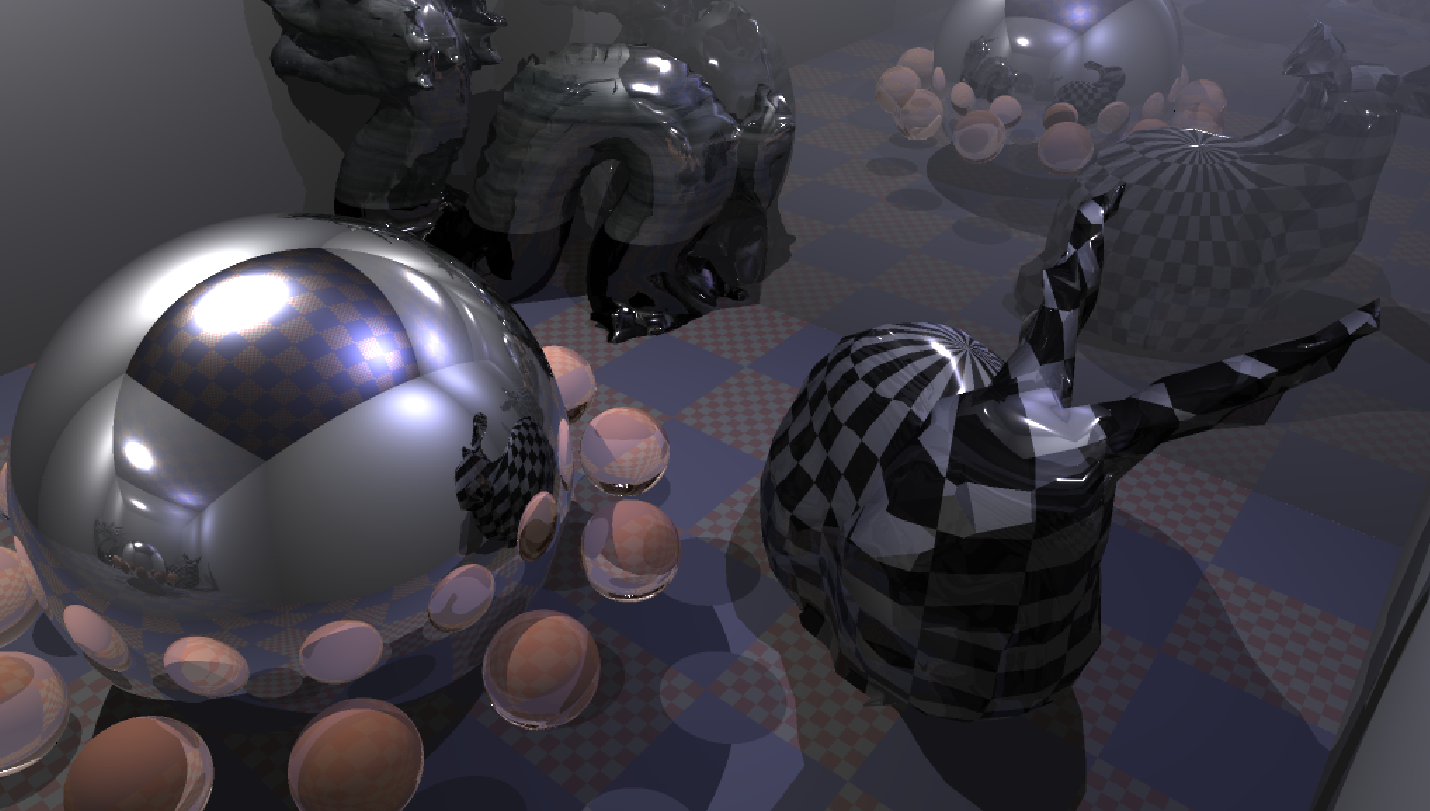
\includegraphics[width=\linewidth]{../screenshots/report_main_1.png}\end{center}
\begin{center}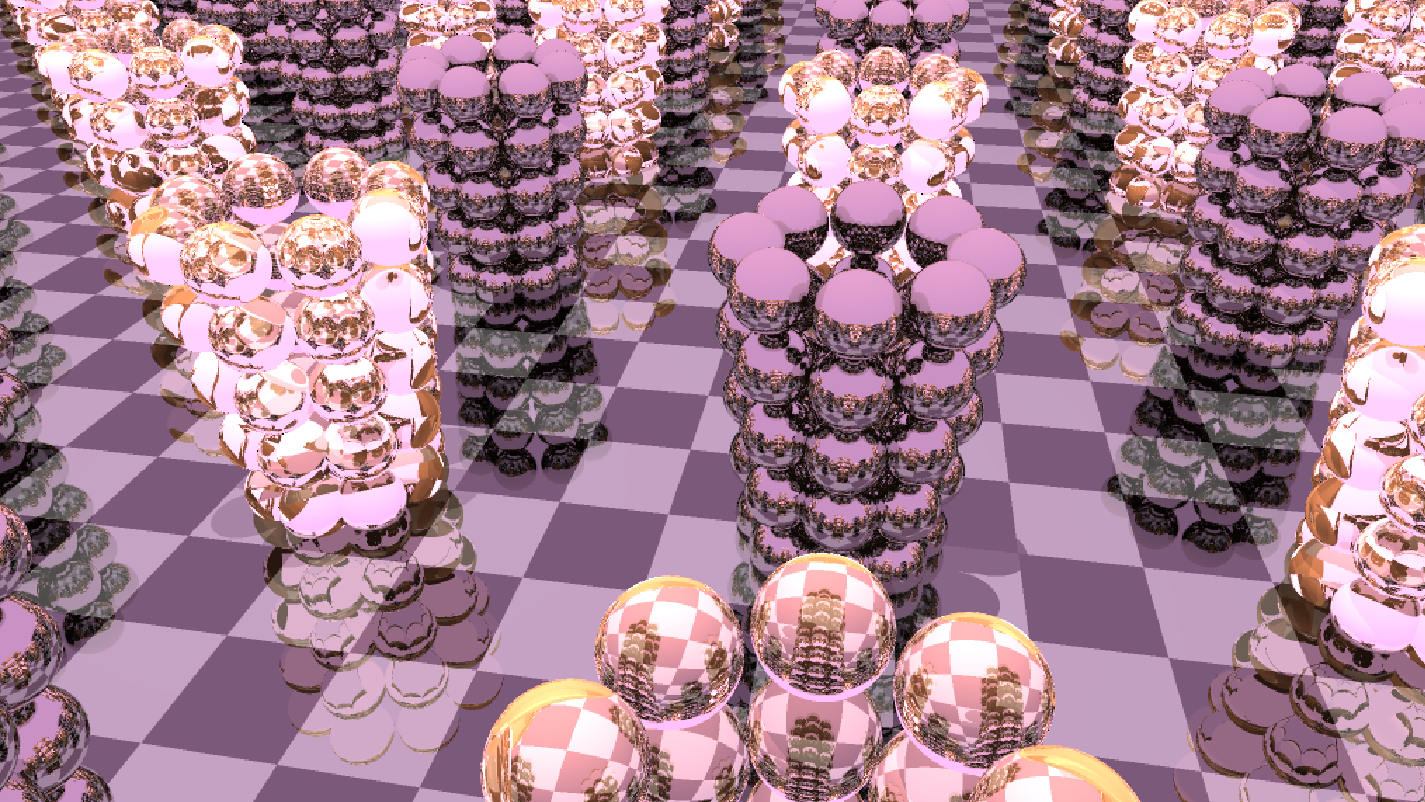
\includegraphics[width=\linewidth]{../screenshots/report_main_2.png}\end{center}

\newpage

\leadin{The renderer}{
The above two images illustrate some of the main features of my ray tracing renderer. The first image was rendered in approximately 12 minutes
on my computer (a 2012 dual-core 2.6GHz laptop), and is 1024 pixels wide with 2x2 supersampling. The dragon has over eleven-thousand triangles. This is not too fast, but fast enough that I could enjoy
watching it being rendered.
 
Lighting-wise, this renderer uses standard Whitted-style recursive ray tracing 
for reflection and refraction, and each geometric object is given a diffuse texture (which can be procedural, constant or unused if purely reflective). Available geometric objects
are spheres, planar quads, triangles, and triangular meshes with optional Phong normals.

The renderer architecture is heavily based off of what is introduced in James Arvo and David Kirk's paper ``A Ray Tracing Kernel'' [1],
and described in detail in the book Physically Based Rendering: From Theory to Implementation, by Matt Pharr and Greg Humphreys. This renderer is definitely not physically based,
but I have used their book as a guide for what abstractions and classes are useful, and, for example, how to implement multithreading.
This is my first C++ program, so I spent a lot of time on cppreference.com and fixing bugs that weren't really anything to do with rendering,
so it was good to see a real implementation in C++ as reference.

\vskip 0.10in
\hrule
\vskip 0.05in
Dependencies: OpenGL 4, GLFW3 (a GLUT alternative), glm, and C++11 support. This project was created on a computer running Linux mint.
I have wanted to make this cross-platform, but have not gotten around to it yet, so the build process is dependent on \textbf{make} and \textbf{g++}.
\vskip 0.10in
\hrule
}

\leadin{Usage, architecture, and interaction}{
    The project is modularized so that it can be recompiled for different ``main programs'' and scenes. Scenes are described procedurally in .cpp
    files in the scenes/ directory. A ``main program'' is what the actual main program hands a Renderer and Scene object it has created, using the
    \textbf{make\_scene()} routine of the linked scene file. This modularization is done so that there can be separate utilities such as a renderer that
    opens no window and writes straight to a PPM file, and an interaction renderer reliant on OpenGL 4.

To compile and use it, go to the project root directory, and, for example, run

\vskip 0.05in
\centerline{\textbf{./run progressive\_view center -r 250 -s 2 -c 1 1 1 0 0}}
\vskip 0.05in

The command-line flag arguments are all optional, and denote a 250-pixel width, 2x2 supersampling, and a camera start position
of (1,1,1) (with azimuth and altitude angles of zero). If not specified, these will default to something probably reasonable.
This command should open a window and an OpenGL context, and put you into the first image, with the towers of reflective and refractive spheres.
On my computer (again, a 2012 dual-core 2.6GHz laptop), this runs reasonably and interactively, albeitly at lower resolution while moving.
\\

Interactivity has been one of the major considerations in this renderer. The feedback loop of interactive rendering is part of the reason why it is so fun,
so from the start I have been working on interaction and performance. Multithreading is used to render the image directly while the main thread streams
a texture through the OpenGL 4 pipeline. Otherwise, while moving around, patterns of blocks will be rendered to the framebuffer in such a way that I hope
gives a sense of interactivity. This does not work all the time, but for some scenes (especially ones without the dragon, in at most 512x512 resolution, sometimes
with 2x2 supersampling), the interactivity works nicely. Here is a picture of it:

\begin{center}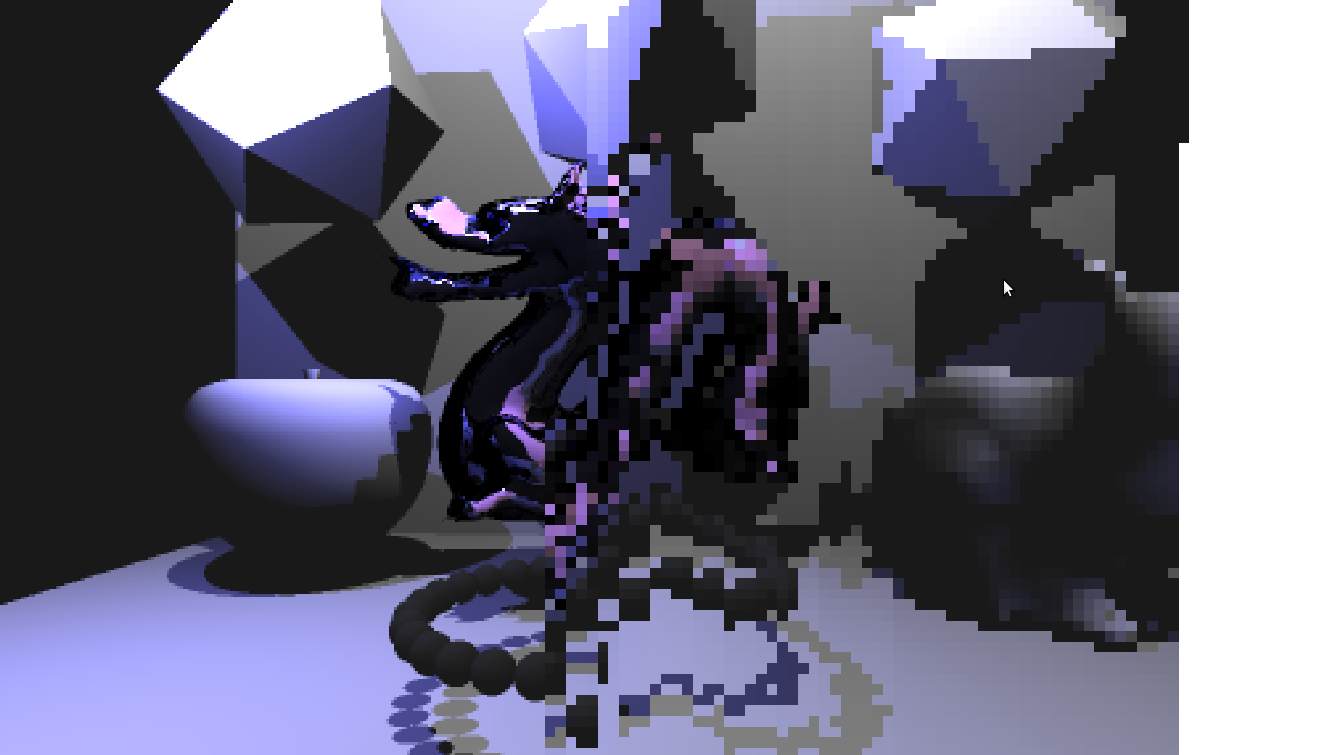
\includegraphics[width=\linewidth]{../screenshots/being_made.png}\end{center}

}
\leadin{Controls when using progressive\_view}{
Press E to toggle the use of the mouse for movement (h,j,k,l or left,down,up,right move the camera if not using the mouse), F to switch modes
(back and forth from pixelated, block-based rendering that attempts to be interactive, to direct rendering, where you can watch as the image is rendered.)
WASD move around as usual, and left-shift moves downward, and space moves upward. Since raw mouse mode is not used, switching between mouse modes with
E allows you to ``drag'' the view.
}

\leadin{Procedural scene description}{

As described before, scenes are described in a C++ source file and linked to a main program (of which I have two, interactive and write-to-file).
This is much simpler than the parsing of a scene description file (as described in the PBR book), and in my case I think this gives a lot more
freedom to describe interesting scenes using arbitrary programming constructs. Here is an example, declaring the checkerboard-textured bunny in the first image:

\VerbatimInput{code2.txt}

As can be seen from the formatting of the code, this is an ideal candidate for some sort of JSON-like format, which is a project I want to do sometime as I am interested
in parsers.
}

\leadin{Mesh rendering}{
Mesh rendering was one of the major features I wanted from the start, and it is very satisfying.
Most modern ray tracing systems apparently tessellate geometry into micropolygons and accellerate their intersection
with things such as bounding volume heirarchies, which I use here. What is great is that along with bounding volume heirarchies,
the complex detail of a mesh only really matters performance-wise when a large part of the model is in view. The below image is the first render I made
with this new ability.
\begin{center}
\includegraphics[width=200pt]{../screenshots/dragons.png}\end{center}
}


\leadin{Procedural and image texturing}{
    There is support for a basic form of ``shade trees''. I hope to later add full support for material descriptions like Cook's shade trees.
    I use this idea for the checkerboard-inside-a-checkerboard texture. The CheckerTexture class holds two pointers to textures, and x and y
    grid extents. A very simple one-liner lets shading calculation be done with alternating textures -- either of which could again be a grid texture
    of higher resolution!
    \VerbatimInput{code1.txt}
}

\leadin{Lighting hack for transparent shadows}
{
    This turned out to look alright in some cases, but appears to break physical law when interacting with other shadows. I will fix this!
}

\leadin{Antialiasing with supersampling}
{
    The supersampling is very simple -- the renderer just writes to a larger framebuffer, and sets some variables to let the system know
    to downsample it when written out to a PPM file or streamed to the screen. The n-by-n block of samples is averaged to give one pixel.
    This gives a definite boost in visual quality, even with 2x2 supersampling, so I have turned it on for most renders, even though it takes
    longer and it is definitely not the most effective technique.
}

\leadin{Bounding volume heirarchies}{
One major feature is bounding volume heirarchies. Implemented without any sort of optimization (as a tree in dynamic memory), these
already substantially increased the performance of the renderer. Further gains in performance were obtained through a compactification
of the tree into a linear array, and a specialized BVH data structure for triangle meshes.
}

\leadin{Multithreading}{
As my first multithreaded program, the code here is a bit of a mess, but it appears to work, and sped up the speed of rendering my main test scene
(a large number of spheres, as shown below) from hovering around 3.459 seconds, to 1.898-2.031 seconds! Multithreading is only used when doing direct rendering,
rather than rendering while moving, since the code for that is already a mess of ``coroutine'' logic which saves state, reuploads the image, and goes back
to whatever blocks it was working on.

\begin{center}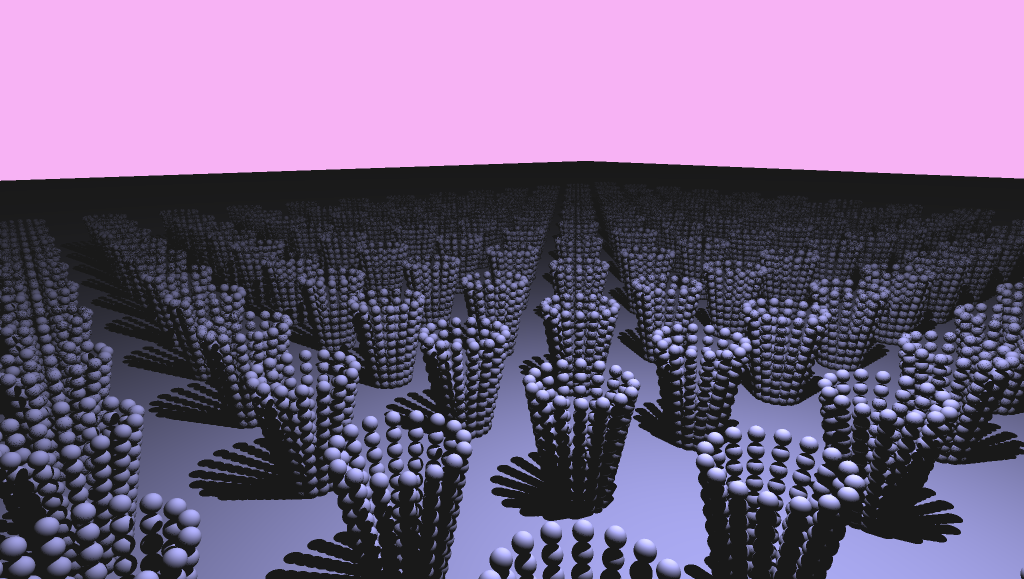
\includegraphics[width=200pt]{../screenshots/more.png}\end{center}

Here I used pbrt (the ray tracer described in the book) as a reference. With multithreading, 16x16 or 32x32 tiles are tasks, which
the threads wait around to grab. Information about the available tile-tasks is necessarily mediated through mutexes and thread-synchronization, using
the C++11 standard thread library. Although there was a definite measured speed up, the program now occassionally segfaults (not too often), and I suspect the
culprit is my horrible threading code. I did want a reason to start learning this though so I am glad I implemented it!
}


I will end this report with a collage of images which I think detail the successes and failures I have encountered while developing this renderer.
There is a lot more I want to do -- I have the complete code for NURBs surfaces in OpenGL 4 working, and am going to add a dicer to this program. Hopefully
I can salvage some of the less because-it-works code in here to develop this into a better renderer. Animation was also one of the first goals I had, which I did not end up finishing (apart from creating a short choppy video of some spheres moving).

\begin{center}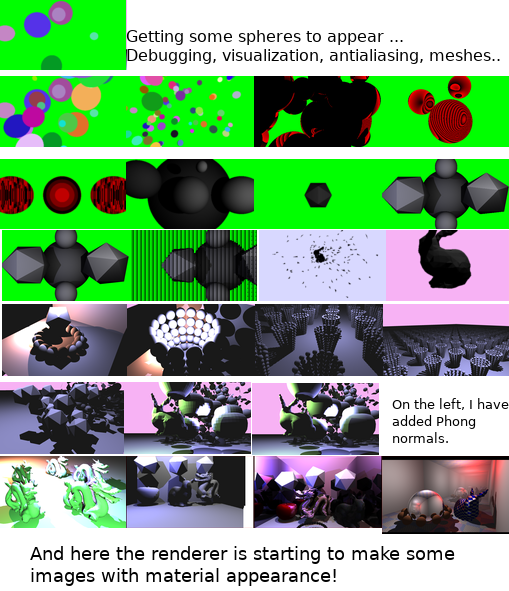
\includegraphics[width=\linewidth]{../screenshots/collage.png}\end{center}

\end{document}

